\chapter{Sampling Sequences In Any Order}
\label{C:a-o-sampling}

The unique properties of transformer models allows great flexibility in the kind of tasks that they can be trained to perform. This chapter shows that with minor changes to the model architecture and training procedure, a probabilistic transformer model is able to generate data in any order, including dynamically choosing the order of the data while sampling. The resulting model is a stochastic process on the dataset.

\section{Introduction}

What is the best order to sample pixels in an image, to maximize the quality of the sample as a whole? Is it unimportant, in which case any order will do? Or does the optimal sampling order depend on the data itself?

To answer this question, a transformer-based neural network model is trained on the MNIST dataset \cite{mnist} so that it can be used auto-regressively sample sequences of pixels in any order.

The model is then used to compare the following sampling orders:
\begin{itemize}
    \item Left-to-right, top-to-bottom
    \item Random
    \item Highest-entropy-first
    \item Lowest-entropy-first
\end{itemize}

Contrary to my hypothesis that a lowest-entropy-first sampling order would result in the best samples, such sampled images are biased towards images with large amounts of empty background, such as images of 1s. Correspondingly, images sampled with highest-entropy-first sampling order are biased towards images of 8s and 9s. In the discussion, I hypothesize this occurs because the criterion we are selecting for introduces a bias, and I characterise this bias.

\subsection{Dynamically-ordered auto-regressive sampling}

If we have an auto-regressive model of the appropriate form that has been appropriately trained, we can dynamically choose the order that we sample a sequence. The form of the model must be such the data can be split into two components `position' and `content' which we will represent with $x_i$ and $y_i$ respectively. Often, the inputs are discrete \textit{tokens}, so $x_i ∈ \mathbb{N}$ and $y_i ∈ \mathbb{Z}$.

A sampling order is a sequence of $i$, and no longer represents the same information as the location $y_i$. Instead, it represents the order in which the sampling procedure will traverse the locations $y_i$.

To dynamically determine a sampling order, we compute the conditional distribution over all candidate locations, then choose only one to sample from. A single step in the process looks as follows: given some total sequence length $N$ and seed sequence length $n$, we have input (seed) data $\x_{≤n} = \{ (x_i, y_i) \mid i ≤ n \}$. (The order of the inputs is unimportant). For each remaining position $x_j$, $j ≥ n$, we can compute the conditional distribution $p(y_j \mid x_j,  \x_{≤n})$. This gives us $N - n$ conditionally-independent distributions.

Given that we have a number of conditionally-independent distributions $p(y_j \mid x_j,  \x_{≤n})$, and we can sample from any of them, which one \textit{should} we sample from? This is the question which the experiment in this chapter tries to answer. We can choose any statistic of these distributions as a heuristic to decide the sampling order. For example, we could choose the distribution with the highest entropy, or the distribution with the lowest entropy, or the distribution with the highest mean, or the distribution with the lowest mean, etc. We can then sample from the chosen distribution to get the next $y_n$.

For the experiments we will compare the following sampling orders:
\begin{itemize}
    \item Fixed order (left-to-right, top-to-bottom)
    \item Random
    \item Highest-entropy-first
    \item Lowest-entropy-first
\end{itemize}

Because the data are being sampled, and the auto-regressive factorization of a sequence is in principle independent of the order of the factorization (as discussed in \Cref{ss:ar-factorization}), we might expect that the order has no effect -- however in practice, the distribution of results may be affected because the model is imperfect, and the sampling process may introduce statistical bias when choosing the next location to sample. This will be discussed more in \Cref{s:a-o-discussion}.

\subsection{Arbitrary order auto-regressive pre-training}
\label{sss:pretraining-triples}

Arbitrary order auto-regressive sequence modeling is a variant of auto-regressive pretraining developed specifically for this project. Let us recall causal/autoregressive pretraining from the previous chapter (see \Cref{fig:pretraining-causal}). Recall that these predict the next input from the previous input, conditioned on the rest of the sequence via their attention layers.

The input sequence can be represented as:
\begin{equation*}
   \x = (y_{<i}, x_{<i}) = ( \{ y_i, y_{i-1}, ..., y_1 \}, \{ x_i, x_{i-1}, ..., x_1 \} )
\end{equation*}
where $i$ represents the index (sampling order), $y_i$ represents the position of a token, and $x_i$ represents the value of a token. When sampling the next input based on the previous input, the model typically infers the next position from the previous position. However, if the data is not in order, then the the model is not able to infer the target position. We instead construct an input sequence in the following way, providing the model with the \textit{target} position information explicitly:
\begin{equation*}
   \x = (x_{<i+1}, y_{<i}, x_{<i}) = ( \{ x_{i+1}, x_{i}, ..., x_2 \}, \{ y_i, y_{i-1}, ..., y_1 \}, \{ x_i, x_{i-1}, ..., x_1 \} ).
\end{equation*}

By providing the input as [target position, input position, input value] triples instead of [input position, input value] pairs (in which the target is implicit), we allow the model to sample the next input value without inferring the next position.

If our sequence was presented in contiguous forward-only ordering, the target position of $x_i$ would always be the same, and so the addition of $x_{i+1}$ would not introduce any new information. However, in this pretraining task we randomly shuffle the order of the tokens, so the model learns to utilize this information.

At inference time we can choose $x_{i+1}$ to be any position that we want the model to sample next, by constructing the following triple $(x_{i+1}, y_i, x_i)$ and appending it to the rest of the previous tokens. This enables performing the experiments with dynamic sampling orders.

\section{Previous work}
\label{s:previous-work}

A stochastic process is a sequence of random variables, where each random variable depends on the previous random variables. Equivalently, a stochastic process is a function drawn from a probability distribution over functions. Stochastic processes are extremely useful objects. One notable use is for Bayesian Optimization (which we will not discuss here), and they are also used in many other areas, such as in the study of dynamical systems, and in the study of random walks.

This section discusses some previous work relating neural networks and stochastic processes, and how it relates to the work in this chapter.

There are a number of previous works that have explored the use of neural networks as stochastic processes:
\begin{itemize}
    \item Neural Processes \cite{neural-processes}
    \item Attentive Neural Processes \cite{attentive-neural-processes}
    \item Transformer Neural Processes \cite{transformer-neural-processes}
    \item Transformers Can Do Bayesian Inference \cite{transformers-bayesian}
\end{itemize}

What these works have in common is that create some kind of learned model which fulfills the properties of a stochastic process. A key aspect that defines a stochastic process is that the distribution over the function space is invariant to permutations of the input sequence, and that the inputs sequence can be of any length. `Neural Processes' use a mean pooling operation to achieve this, but the subsequent works use the attention operation to achieve this.

The models can be used draw samples from any point in a function space, then can be conditioned on the newly sampled points to form a new learned distribution over the same function space.

The main difference between current approaches to neural stochastic processes is which family of distributions the learned model uses. In `Neural Processes' and `Attentive Neural Processes', the model consists of two parts in sequence, which we can call $f$ and $g$. The first part  predicts a distribution (typically a multidimensional Gaussian) over latent variables given a set of inputs:
\begin{align*}
    (\mbfmu, \Sigma) = f(\x) \\
    \mathbf{z} \sim \N(\mbfmu, \Sigma),
\end{align*}
and the second part predicts an output given a sampled latent and any target position:
\begin{align*}
    \mathbf{y} = g(\mathbf{z}, \mathbf{x}).
\end{align*}
In other words, the model is a distribution which can be used to sample a latent $\mathbf{z}$ which determines a function from $\mathbf{x}$ to $\mathbf{y}$.

In `Transformer Neural Processes', and `Transformers Can Do Bayesian Inference', the model $f$ outputs the parameters $\mbfvarphi$ for a distribution $q$ (of any functional form) directly:
\begin{align*}
    \mbfvarphi &= f(\x) \\
    \mathbf{y} &\sim q(\mbfvarphi).
\end{align*}
However, due to the difficulties of representing distributions over high-dimensional data, $q$ is typically limited to using an auto-regressive factorization of the distribution:
\begin{align*}
    \mbfvarphi_i &= f(\x_{≤i}, \mathbf{y}_{<i}) \\
    \mathbf{y}_i &\sim q(\mbfvarphi_i).
\end{align*}

These two classes of approach are both equivalent to a stochastic process, but the approach taken in `Neural Processes' and `Attentive Neural Processes' is limited to only sampling, whereas the approach taken in `Transformer Neural Processes', and `Transformers Can Do Bayesian Inference', while limited to an auto-regressive factorization, can be used for computing the entropy, probability density, etc.

The work in this chapter takes the second approach -- learning a function which outputs distributions. Because this approach gives access to closed-form distributions, it is possible to compute the entropy, probability density, and other quantities of interest. This is not possible with the other approach, which only enable sampling from the distribution. However, the other approaches are able to learn more complex distributions.

The above works \cite{transformer-neural-processes} and  \cite{transformers-bayesian} are the most similar to the work in this chapter. The model trained in this chapter is exactly a `Transformer Neural Process', except that the model in this chapter outputs discrete distributions rather than Gaussian distributions.

The work in this chapter investigates the effect of choosing a dynamic sampling order for image completion with a transformer neural process based on the entropy of the distribution. To my knowledge none of the previous works have investigated this.

\section{Hypothesis}
\label{s:a-o-hypotheses}

By training a transformer model with the pretraining method described in \Cref{sss:pretraining-triples}, we get a model which can be used to sample any position in the image. We can then use this model to sample the image in different orders, and compare the results.

Using the model we can choose a dynamic ordering in which to sample a sequence at inference time. In particular, one of the ways we can do this is by evaluating the \textit{entropy} of all candidate positions, then sampling from the one with either the lowest or the highest entropy.

My hypothesis was that when auto-regressively sampling pixels to produce MNIST images, using a ``lowest-entropy-first'' ordering will produce visually better results than a ``highest-entropy-first'' ordering.

\section{Method}

To investigate this hypothesis, a transformer neural process was trained with the pretraining method described in \Cref{sss:pretraining-triples}, on the MNIST dataset. The model was then used to sample images in different orders, and the results were compared.

\subsection{Data}

This series of experiments uses the MNIST dataset, which is a set of 28x28 grayscale images of handwritten digits. The dataset was split into a training set of 60,000 examples, and a test set of 10,000 examples. Each image is labeled with the digit it represents, from 0 to 9, but the labels were not used in the experiments. Each pixel is represented as a value between 0 and 255, where 0 is black and 255 is white.

Instead of representing full 256 gray levels, a 2-bit representation was used, where each pixel is represented as a value between 0 and 3. The 256 levels were discretized further into 4 levels using a learned k-means clustering over the all pixel values in the MNIST training set. This was done to simplify the form of the distribution that the model would output, and remove any complextity here as an additional variable to debug. 4 levels was the smallest representation that gave good visual quality when the images were reconstructed.

The MNIST images were then formatted into a sequence prediction task using the following procedure. First, each image was treated as a sequence of $28\times28 = 784$ triplets, where each triplets contains three integers: the row index of the pixel and the column index of the pixel (both in the range $[0, 28)$), and the pixel value (in the range $[0, 4)$ -- 0 = black, 1 = dark gray, 2 = light gray, and 3 = white).

The sequence of triplets was then shuffled to form a random permutation of the pixels. The row and column indices of each pixel were then appended to the previous triplet, forming a 5-tuple. This was done to specify the target position that the model should predict, which it could no longer infer from the ordering of the sequence since the sequence was shuffled.

Lastly, all of the integers each 5-tuple were embedded using learned codebooks, and the resulting sequence of embedding vectors was used as the input to the model.

Some examples of this task are shown in \Cref{fig:mnist-task-examples}.

\begin{figure}
    \centering
    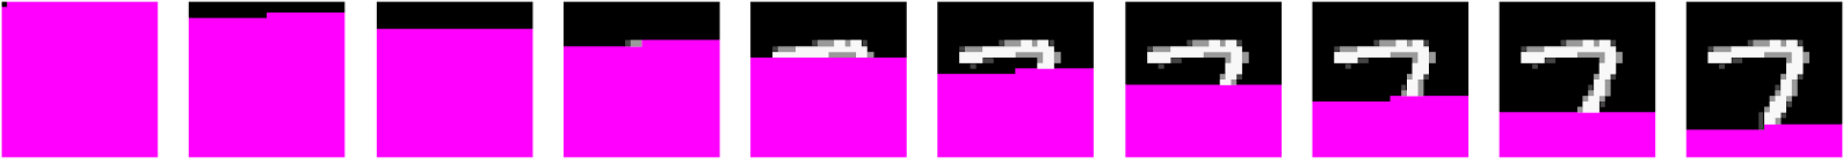
\includegraphics[width=0.7\linewidth]{figures/examples-sequential.png}
    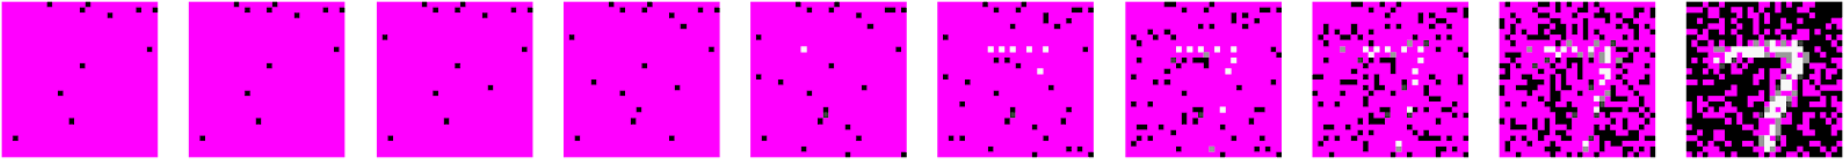
\includegraphics[width=0.7\linewidth]{figures/examples-random.png}
    \captionsetup{parskip=7pt}
    \caption[Examples of the MNIST training task]{Examples of two tasks, showing input sequences with progressively more pixels filled in. (Pink means the pixel was not provided).

    Top: Pixels presented in a contiguous, forward-only order.

    Bottom: Pixels are presented in a non-contiguous, random order. This is the task that the model in this experiment was trained on.}
    \hrulefill
    \label{fig:mnist-task-examples}
\end{figure}

\section{Training}

A transformer model was then trained on the described task. A table of training details is shown in \Cref{tab:training-details}.

\begin{table}[h]
    \centering
    \begin{tblr}
        {
            vlines,
            rows={m},
        }
        \hline
        N° embedding dims & 256 \\
        N° layers & 5 \\
        N° hidden dims & 515 \\
        N° attention heads & 12 \\
        Total N° parameters & 17,495,809 \\
        Batch size & 32 \\
        Sequence length & 784 \\
        Training time & 1h 27m 4s \\
        Training steps & 20,000 \\
        \hline
    \end{tblr}
    \caption[Training details of MNIST model]{Training details for the probabilistic 4-color model.}
    \hrulefill
    \label{tab:training-details}
\end{table}

\section{Results}

\begin{figure}
    \centering
    \begin{minipage}{0.8\linewidth}
        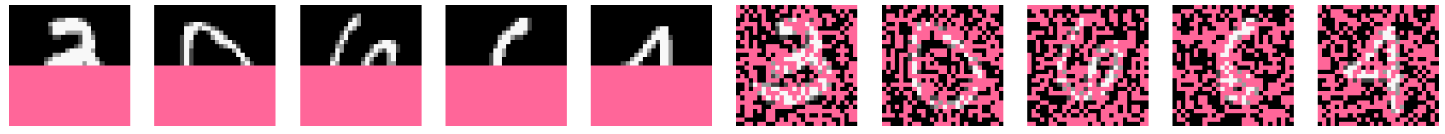
\includegraphics[width=\linewidth]{figures/mnist-4col-seed.png}

        \vspace{0.5cm}

        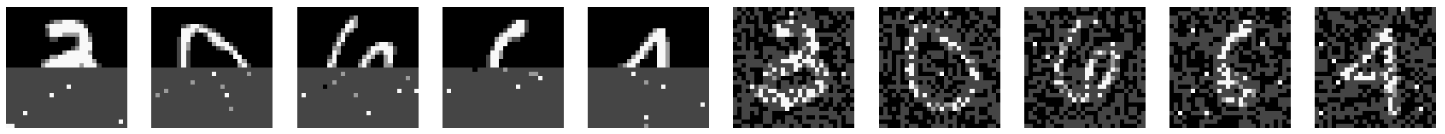
\includegraphics[width=\linewidth]{figures/mnist-4col-0.png}
        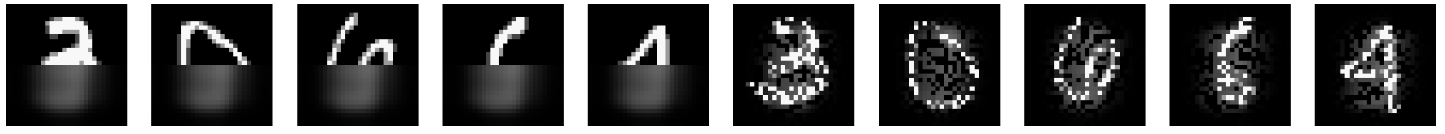
\includegraphics[width=\linewidth]{figures/mnist-4col-1.png}
        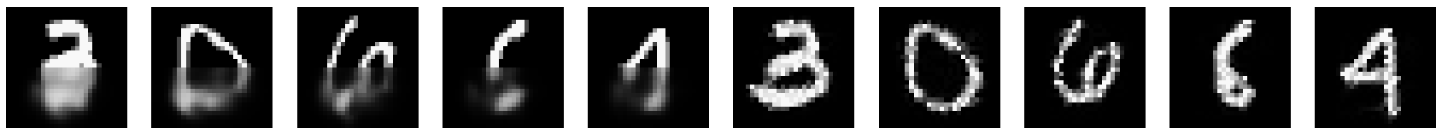
\includegraphics[width=\linewidth]{figures/mnist-4col-2.png}
        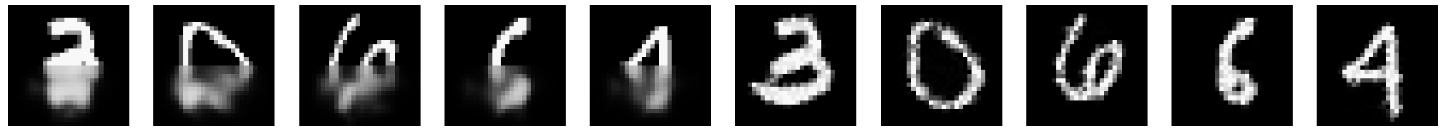
\includegraphics[width=\linewidth]{figures/mnist-4col-3.png}
        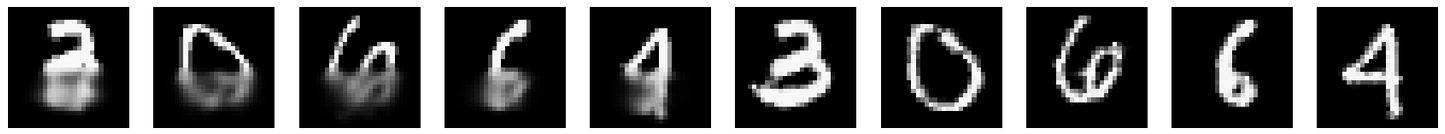
\includegraphics[width=\linewidth]{figures/mnist-4col-4.png}
        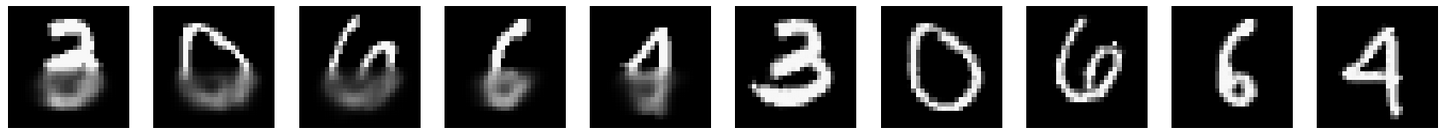
\includegraphics[width=\linewidth]{figures/mnist-4col-5.png}
        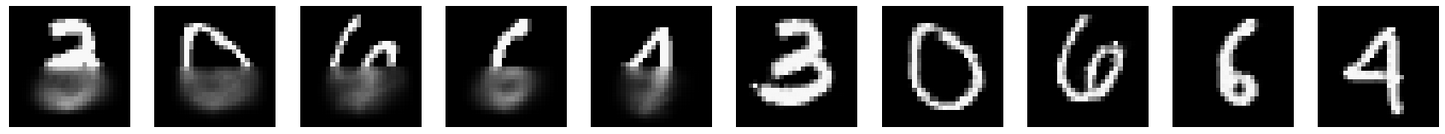
\includegraphics[width=\linewidth]{figures/mnist-4col-6.png}

        \vspace{0.5cm}

        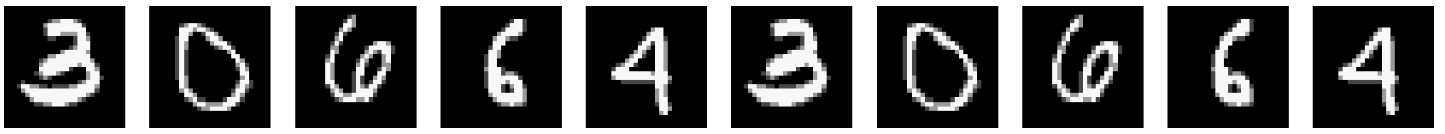
\includegraphics[width=\linewidth]{figures/mnist-4col-targ.png}
    \end{minipage}
    \captionsetup{parskip=7pt}
    \caption[Visualization of convergence during training]{The above figure shows the probabilistic 4-color model converging as it is trained. This was the model used for the sampling order experiments.

    Top: Seed inputs provided to the model. Pink pixels represent inputs not provided.

    Middle, descending: The expected value of the model's distribution over the unknown values as the training process progresses.

    Bottom: Ground truth images.}
    \label{fig:training-4col}
\end{figure}

\begin{figure}
    \centering
    \begin{minipage}{0.8\linewidth}
        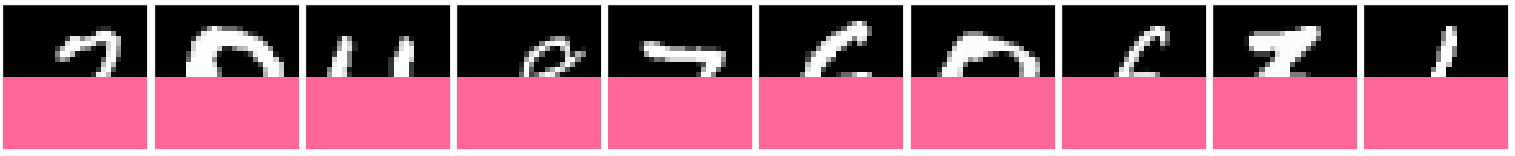
\includegraphics[width=\linewidth]{figures/mnist-training-seed.png}

        \vspace{0.5cm}

        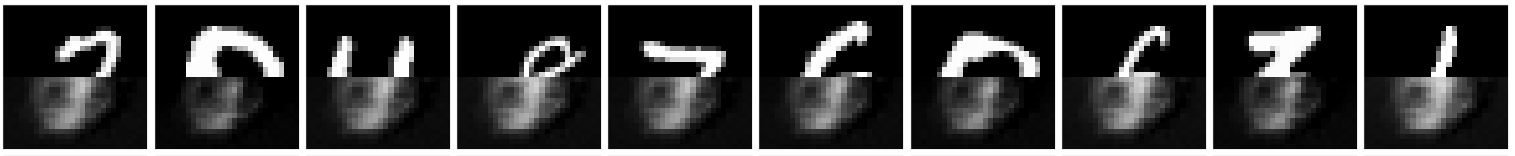
\includegraphics[width=\linewidth]{figures/mnist-training-0.png}
        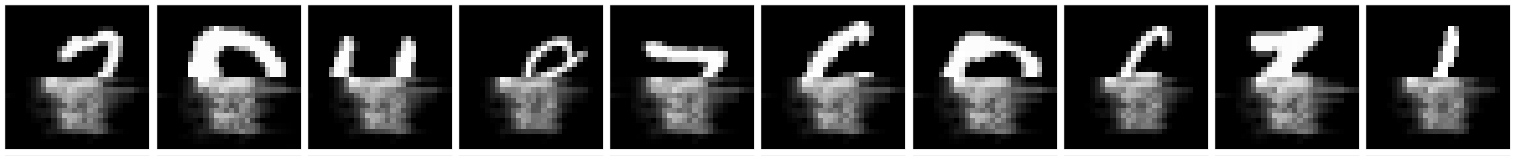
\includegraphics[width=\linewidth]{figures/mnist-training-1.png}
        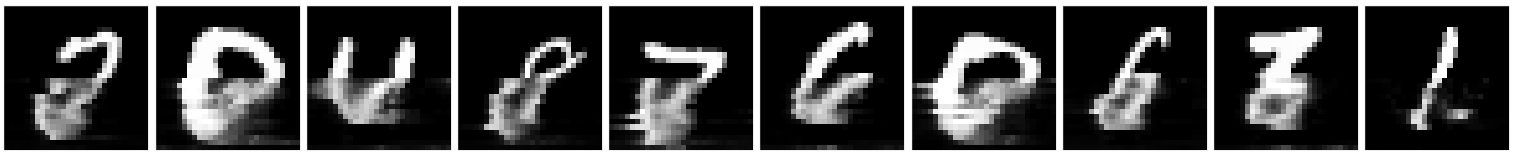
\includegraphics[width=\linewidth]{figures/mnist-training-2.png}
        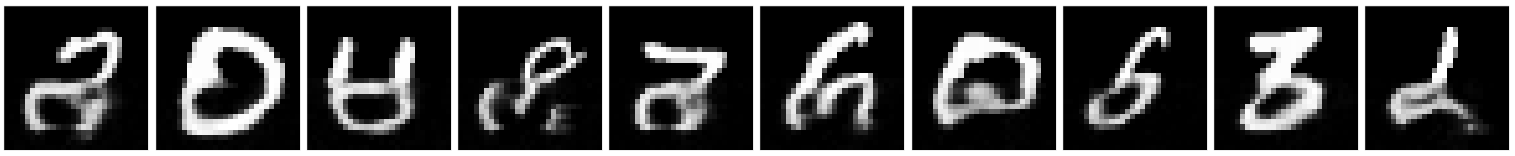
\includegraphics[width=\linewidth]{figures/mnist-training-3.png}
        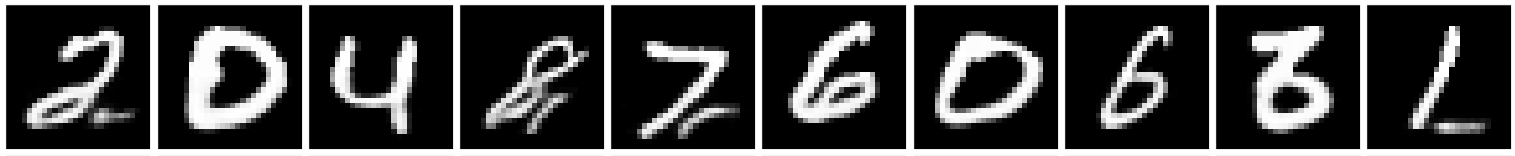
\includegraphics[width=\linewidth]{figures/mnist-training-4.png}
        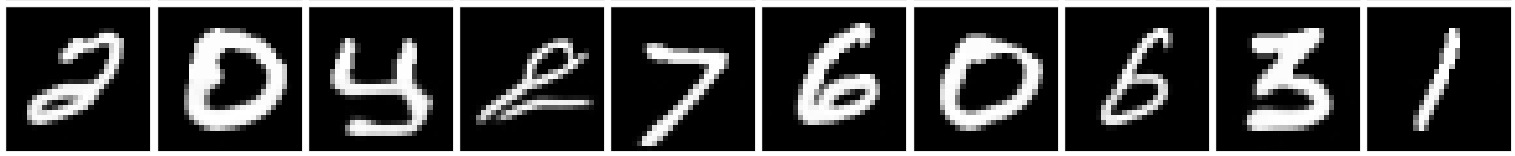
\includegraphics[width=\linewidth]{figures/mnist-training-5.png}

        \vspace{0.5cm}

        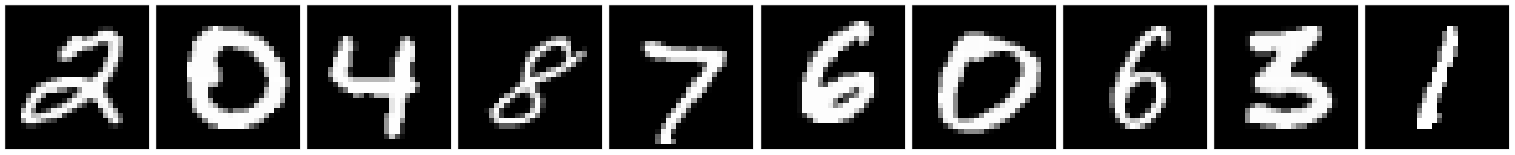
\includegraphics[width=\linewidth]{figures/mnist-training-target.png}
    \end{minipage}
    \captionsetup{parskip=7pt}
    \caption[Visualization of convergence during training]{The above figure shows a deterministic model converging as it is trained. This model predicts the pixel values as a floating point value directly, rather than as a probability distribution.

    Top: Seed inputs provided to the model. Pink pixels represent inputs not provided.

    Middle, descending: The model's prediction over the unknown values as the training process progresses.

    Bottom: Ground truth images.}
    \label{fig:training-deterministic}
\end{figure}

Some predicted images using this model are shown in \Cref{fig:training-4col}. For comparison, a deterministic model trained on a standard forward-only autoregressive pretraining task is shown in \Cref{fig:training-deterministic}. The deterministic model was trained for the same number of steps, and with the same hyperparameters as the probabilistic model, but was trained on a different task and with a different loss function.

\begin{figure}
    \centering
    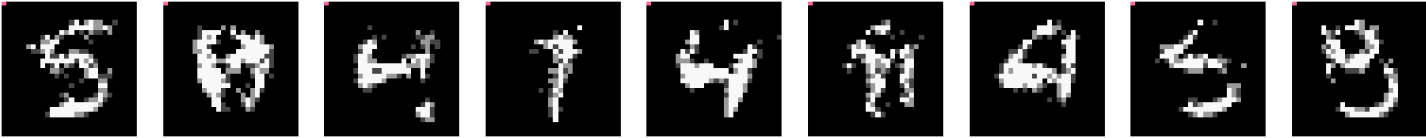
\includegraphics[width=0.8\linewidth]{figures/samples-sequential.png}
    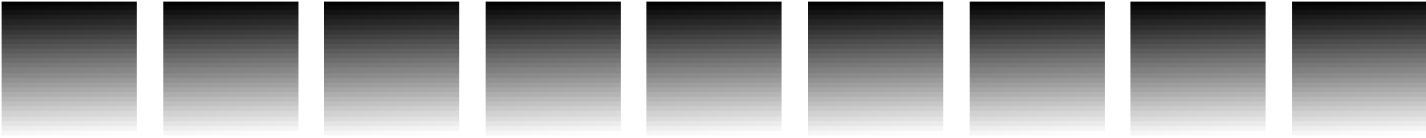
\includegraphics[width=0.8\linewidth]{figures/sampling-order-sequential.png}

    \vspace{0.7cm}
    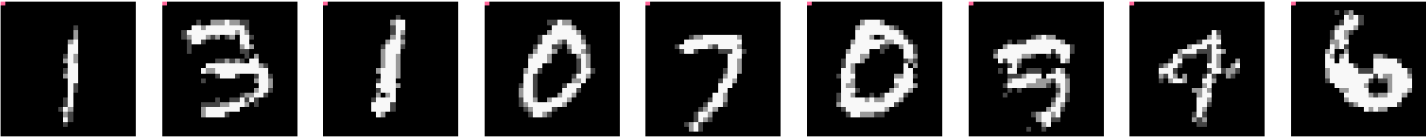
\includegraphics[width=0.8\linewidth]{figures/samples-random.png}
    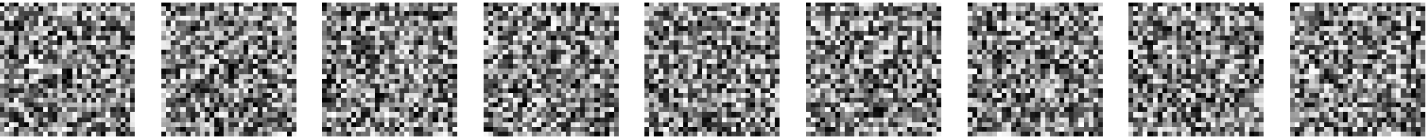
\includegraphics[width=0.8\linewidth]{figures/sampling-order-random.png}

    \vspace{0.7cm}
    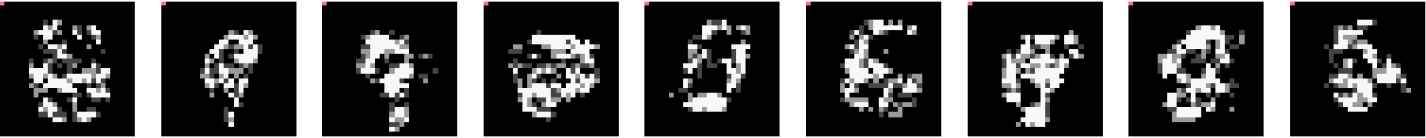
\includegraphics[width=0.8\linewidth]{figures/samples-high-entropy.png}
    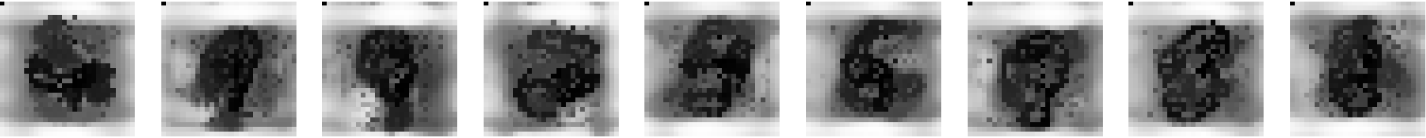
\includegraphics[width=0.8\linewidth]{figures/sampling-order-high-entropy.png}

    \vspace{0.7cm}
    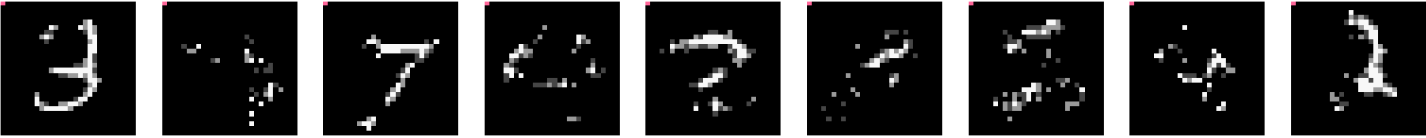
\includegraphics[width=0.8\linewidth]{figures/samples-low-entropy.png}
    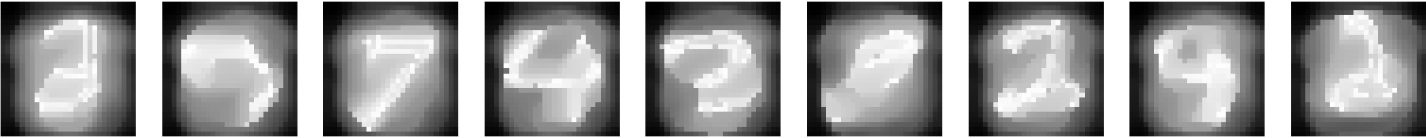
\includegraphics[width=0.8\linewidth]{figures/sampling-order-low-entropy.png}
    \captionsetup{parskip=7pt}
    \caption[Visualization of predicted images with different sampling orders]{The above figure shows the effect of the sampling order on the visual quality of the predicted images, using the probabilistic 4-color model. Each pair of rows shows predicted images and a visualization of the sampling order used to generate it, respectively. The bottom row of each pair is a visualization of the sampling order, where the color of each pixel indicates the order in which it was sampled -- black pixels were sampled first, and white pixels were sampled last.

    Top: Sequential sampling order, where pixels are sampled in the order they appear in the image.

    Top-middle: Random sampling order, where pixels are sampled in a random order.

    Bottom-middle: Highest-entropy-first sampling order, where pixels are sampled in order of decreasing entropy.

    Bottom: Lowest-entropy-first sampling order, where pixels are sampled in order of increasing entropy.}
    \label{fig:order-comparison}
\end{figure}

The results of using the model to sample images using different sampling orders are shown in \Cref{fig:order-comparison}.

\section{Discussion}
\label{s:a-o-discussion}

As we can see in \Cref{fig:order-comparison}, the ``lowest-entropy-first'' ordering produces distinct images from the ``highest-entropy-first'' ordering. However, neither is as good as the ``random'' ordering. This clearly disproves the hypothesis that the ``lowest-entropy-first'' ordering would produce the best results.

Why do the ``lowest-entropy-first'' and ``highest-entropy-first'' orderings produce such different results? Why should they be different from the ``random'' ordering?

If the model has perfectly learned the true distribution of the data, then all orderings should produce the same results, because the order of an auto-regressive factorization is in theory unimportant (see \cref{eqn:ar-factorization-random}). However, the model is not perfect, and the ``random'' ordering is the only one that is not biased by the model's imperfections.

When we select a dynamic ordering based on the model's predictions, we are introducing a bias into the model's predictions. Let us examine this bias in more detail.

Let us imagine that the model outputs a Gaussian -- more specifically it outputs estimates of the parameters $\mu$ and $\sigma$ of the true conditional distribution $p(y_i \mid x_i, y_{<i}, x_{<i})$. Then, also assume we can approximate the the fact that the model is imperfect by adding Gaussian noise to the model's output, $\mu + \epsilon_\mu$ and $\sigma + \epsilon_\sigma$, where $\epsilon_\mu \sim \N(0, v_\mu)$ and $\epsilon_\sigma \sim \N(0, v_\sigma)$, for some small $v_\mu$ and $v_\sigma$. Let the model's output distribution be $q(i) = \N(y_i | x_i, y_{<i}, x_{<i}, \mu + \epsilon_\mu, \sigma + \epsilon_\sigma)$.

If we select the next position $i$ randomly, then when we sample $y_i \sim q(i)$, since the means of the error terms $\epsilon_\mu$ and $\epsilon_\sigma$ are both 0, the expected value of $y_i$ remains $\mu$.

However, when we select the next location $i$ to sample based on the entropy of $q(i)$, we select the location among many which has the highest (or lowest) variance $\sigma + \epsilon_\sigma$. On average, we will select a position with both high contribution from $\sigma$, \textbf{and} high contribution  from $\epsilon_\sigma$. Because of the high $\epsilon_\sigma$ term, this selection biases us towards sampling from distributions where the model is more uncertain than in the true distribution. We will therefore draw samples that are on average \textbf{less likely} in the true distribution. i.e. $\E[p(y_i \mid x_i, y_{<i}, x_{<i})] < \E[q(i)]$. To summarize, when we select an $i$ because the corresponding $q(i)$ has high entropy (variance), and then sample from this distribution, we will produce a pixel with a value that has $p(y) < q(y)$. The reverse is true for the ``lowest-entropy-first'' ordering. The selected locations are biased towards areas where the model has incorrectly low $\epsilon_\sigma$, ie. is incorrectly over-confident, and the resulting samples are higher probability in the predicted distribution, but (assuming also non-zero $\epsilon_\mu$) lower probability in the true distribution than unbiased samples. This is the bias that we are introducing into a \textit{single} prediction from the model.

I claim this same reasoning applies for the discrete case which I actually used in the experiment -- we can add an $\epsilon$ term to the logits, which when selecting for high entropy, pushes them towards the uniform distribution, and when selecting for low entropy, pushes them away. It so happens that on MNIST, this typically means the pixel will be brighter.

As we repeat this process, we will produce some pixels that are on average brighter than the true sequence. When the model is conditioned on these, it will generally infer that the remaining pixels should be brighter as well. This is why the ``highest-entropy-first'' ordering produces images that are as a whole brighter than the ``lowest-entropy-first'' ordering, and why both are shifted away from the ``random'' ordering.

\section{Conclusions and Future Work}
\label{s:a-o-conclusions}

In this chapter, we have shown that the order in which we sample from a model can in practice have an impact on the quality of the samples produced, despite different sampling orders being equivalent in principle (\Cref{eqn:ar-factorization-random}). However we also showed that sampling with ``lowest-entropy-first'' and ``highest-entropy-first'' produce a directional bias in the samples produced. This bias is due to the fact that the model is imperfect, and selecting locations based on the entropy has the effect of compounding these imperfections. With some assumptions about the nature of these imperfections, we showed that sampling with a ``highest-entropy-first'' ordering shifts the samples towards the uniform distribution, and sampling with a ``lowest-entropy-first'' ordering shifts the samples away from the uniform distribution.

Future work could explore the effect of this bias under different classes of probability distributions, and investigate other sampling orders such as a learned order.
